\chapter{Problem Statement}
HTTP/1.1 was first documented in RFC 2068 \cite{b9} and since its inception, it supports sending multiple HTTP requests over the same TCP or SSL/TLS socket. The HTTP requests are sent back to back and the server uses the HTTP headers to identify where a request ends and the subsequent request starts. \\\\
Consider an architecture composed of a chain of systems as depicted in Figure \ref{fig:HTTP Desync Attack}. Here we see an extreme necessity of synchronization between the frontend and the backend. The frontend and backend have to agree where a request starts and where it ends. If a malicious user or a hacker is able to deceive these systems into disagreeing about the start and end points of a request, it gives him/her the ability to send mailicious message (\textcolor{red}{Red} coloured message in Figure \ref{fig:HTTP Desync Attack}) as part of the request. This malicious message gets appended at the start of the next user`s request. The malicious message appended to other user's requests are carefully designed to carry out attacks on the host systems. 

\textbf{Note : }In all the further examples we consider, the colour of the requests (\textcolor{mygreen}{Green}, \textcolor{myred}{Red} and \textcolor{myorange}{Orange}) in Figure \ref{fig:HTTP Desync Attack} will correspond to the color of the text in the examples. 
\begin{figure}
	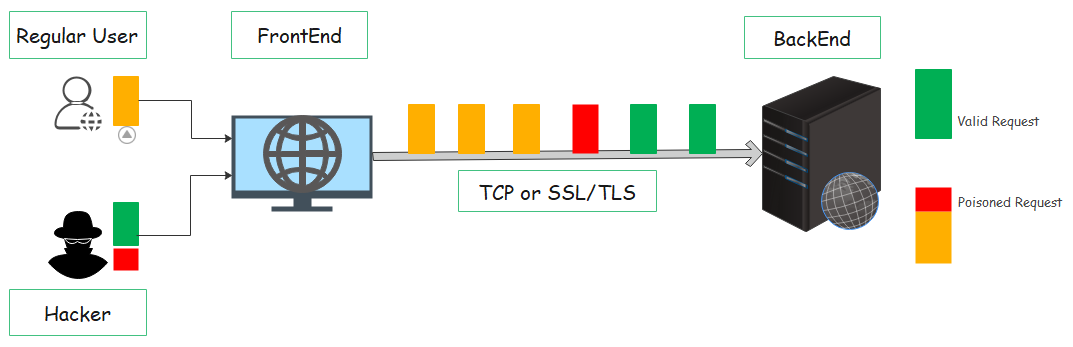
\includegraphics[width=14cm]{images/HTTP_Desync}
	\caption{HTTP Desync Attack}
	\label{fig:HTTP Desync Attack}
\end{figure}


